\section{Resultados Esperados \label{resultados_esperados}}

Nesta Se��o � demonstrada algumas imagens que representam os
resultados finais esperados.

A Figura \ref{img:resultados_preview1}, representa a a��o de o editor
adicionar um novo v�deo ao projeto.
Caso ele queira que as transi��es sejam detectadas, ele seleciona "OK", caso
contr�rio, "Cancel".

\begin{figure}[h|top]
 \centering
 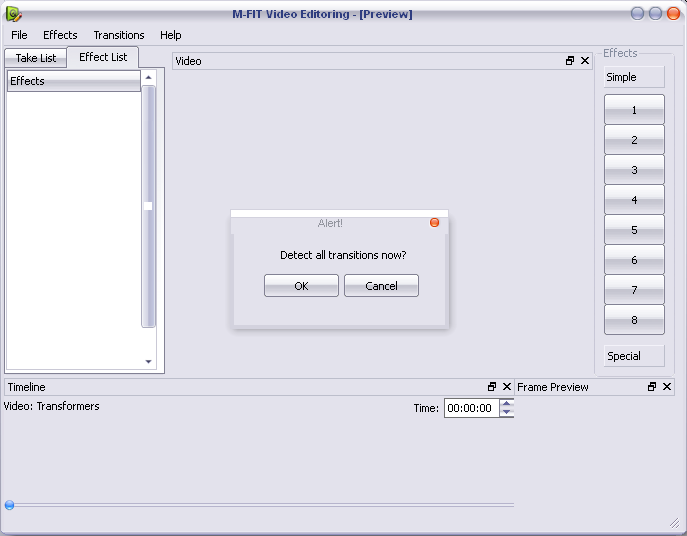
\includegraphics[width=1.0\linewidth]{imagens/resultados_preview1.png}
 \caption{Interface de abertura de um novo V�deo.}
 \label{img:resultados_preview1}
\end{figure}

Se a op��o de escolha foi o "Cancel", o sistema n�o detectar� as transi��es,
e a �rea de trabalho do editor ser� aberta com alguns elementos faltantes.
O editor pode a qualquer momento desejar que as transi��es sejam detectadas.
Ele faz isso acessando o menu "Transition" e escolhendo que tipo de transi��o
ele deseja que seja detectado. Este tipo de procedimento pode ser realizado
caso o editor queira que somente transi��es do tipo corte (exemplo) sejam detectadas.
Este exemplo pode ser verificado na Figura \ref{img:resultados_preview2}.

$\newline$

\begin{figure}[h|top]
 \centering
 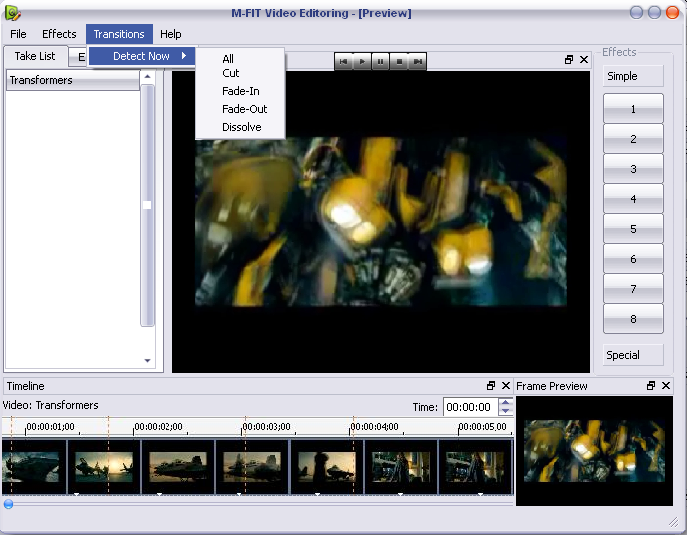
\includegraphics[width=1.0\linewidth]{imagens/resultados_preview2.png}
 \caption{Area de trabalho sem ter as transi��es detectadas.}
 \label{img:resultados_preview2}
\end{figure}

Se a op��o de escolha foi o "OK", o sistema realizar� a detec��o de todas
as transi��es no v�deo, e exibir� a mesma na forma de uma lista para o 
editor. O editor ent�o tem a possibilidade de selecionar uma das v�rias
tomadas da lista, delimitando-as assim na timeline. Esta vis�o pode ser
visualizada na Figura \ref{img:resultados_preview3}.


\begin{figure}[h|top]
 \centering
 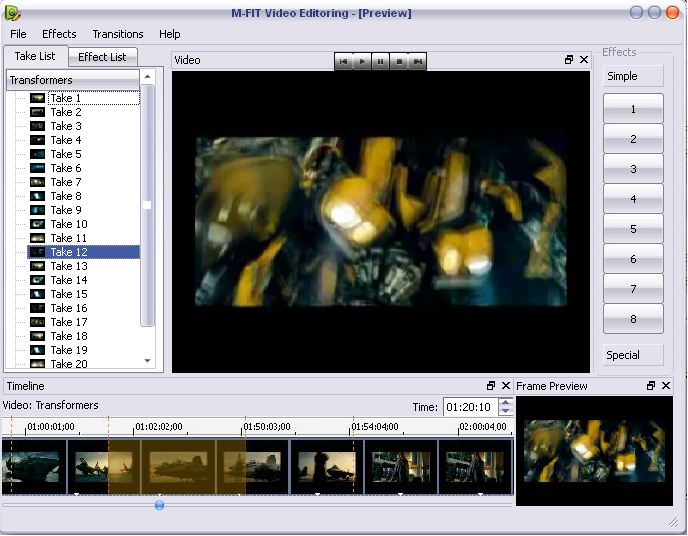
\includegraphics[width=1.0\linewidth]{imagens/resultados_preview3.png}
 \caption{Area de trabalho com as transi��es detectadas.}
 \label{img:resultados_preview3}
\end{figure}
